\documentclass[t]{beamer}
% If you don't have access to the Imperial College beamer theme, then
% commenting out the following line will produce a generic version of the
% slides. 
\usetheme{iclpt}

\usepackage{color,listings}
\usepackage{pstricks, pst-node}
\usepackage{pgfpages,xspace,array}

\newcommand{\doc}[1]{\psshadowbox[framearc=0]{#1}}
\newcommand{\program}[1]{\psframebox[framearc=.2]{#1}}

\usepackage{graphicx,stmaryrd,cancel}
\usepackage{bibentry}
\usepackage{natbib}
\usepackage{hyperref}
\usepackage{amscd}
\usepackage{booktabs}
\bibliographystyle{elsarticle-harv}
\usepackage{amsmath}

\renewcommand{\vec}[1]{\boldsymbol{#1}}

\lstset{frame=single}

\expandafter\ifx\csname natexlab\endcsname\relax\def\natexlab#1{#1}\fi
\expandafter\ifx\csname url\endcsname\relax
  \def\url#1{\texttt{#1}}\fi
\expandafter\ifx\csname urlprefix\endcsname\relax\def\urlprefix{URL }\fi

\definecolor{icdarkblue}{RGB}{23,18,134}
\definecolor{icdarkgreen}{RGB}{0,130,0}

%\setbeameroption{show notes on second screen}

\author[David A. Ham]{Dr David~A.~Ham} 
\date{24 May 2013}

\title{Verification and validation of simulation software}
                  
\institute[Imperial College London]{
  Department of Computing, Imperial College London\\
  Grantham Institute for Climate Change, Imperial College London
david.ham@imperial.ac.uk}

\begin{document}
\nobibliography{bibliography}

\begin{frame}{}
  \vfill{}

  \centering

  \Large\color{icdarkblue}\inserttitle\\
  %\normalsize\insertsubtitle\\[3ex]
  \small\color{black}\insertauthor\\[3ex]
  \footnotesize\insertinstitute

  \vfill{}

  With much material from \bibentry{Farrell2011}

\end{frame}

\begin{frame}{How do we know whether to believe the output of a model?}
  \vfill{}

  \pause
  This is fundamentally a mixed question of mathematics, software
  engineering, and application science. 
  \vfill{}

  \pause
  It's also a critical question which all computational scientists have to
  answer if they expect other scientists or society at large to take note of
  their results.
  \vfill{}
  

\end{frame}

\begin{frame}{A brief trip back to philosophy of science 101}
  
  \begin{itemize}
  \item Mathematical results are \emph{proven}. In other words, if the
    assumptions of a theorem are satisfied, then the result \emph{always}\
    follows. There is no possibility of another result.
  \item Science proceeds by \emph{hypotheses}. These can never be proven in
    the mathematical sense, but they can be \emph{falsified}\ through a
    contrary observation\footnote{\bibentry{popper1959},\\\bibentry{howden1976}}.
  \end{itemize}
  
  So what hypotheses does our software present?

\end{frame}

\begin{frame}{Verification and validation operations}

  \includegraphics[width=\textwidth]{output/verification.pdf}
  
\end{frame}

\begin{frame}{Verification and validation operations}
  
  \begin{itemize}
  \item Only the discretisation of the PDE is usually a mathematical
    operation which can be proven.
  \item Verification of software by mathematical methods is practiced in
    some fields of computing, but simulation code is typically far beyond
    their scope.
  \item The relationship between the continuous model and the physical
    system cannot be directly measured, so we must go through \emph{all}\
    the other steps. 
  \end{itemize}
  
\end{frame}

\begin{frame}{If it's not tested, it's broken.}
  
  \begin{description}
  \item[Unit tests] Tests of correct behaviour applied to the smallest
    possible unit of code.
  \item[Analytic solutions] Very strong tests of correctness of numerics and
    implementation, if you can get one!
  \item[Method of manufactured solutions] A mechanism for generating
    analytic solutions.
  \item[Regression tests] Tests against a previously computed result. Only a
    test of change, not of correctness.
  \item[Third party solution] Tests against another model. Better than
    regression tests, but only as good as the other model.
  \item[Comparisons to ``real'' data] Essential in validating a model, but of
    limited use in verification.
  \end{description}

\end{frame}

\begin{frame}{Some PDE testing theory}

  First, know what convergence means for your numerics. Numerical schemes
  for PDEs usually have convergence behaviour given by an expression such
  as:
  \begin{equation}
    E_h=O(h^n)
  \end{equation}
  Where $E_h$ is the error in the numerical solution, $h$ is a measure of the
  mesh spacing and $n$ is the order of convergence of the method.
  
  It is important to understand both sides of this expression.

  \hfill{}

  Testing convergence behaviour of numerical schemes is a very sensitive
  verification test, since almost any error in the numerics will degrade the
  convergence order.\footnote{At least for schemes of greater than first order.}

\end{frame}

\begin{frame}{Definition of error}
  
  Finite volume and finite element schemes converge in (at least) the space
  $L^2$. So the definition:
  \begin{equation}
    E_h = \left(\int_\Omega(\hat{S}-S)^2\mathrm{d}V\right)^{\frac{1}{2}}
  \end{equation}
  is often appropriate. Here $\Omega$ is the solution domain, $\hat{S}$ is
  the numerical solution and $S$ is the exact solution.
  \vfill{}
  
  Importantly, this is \emph{not}\ the same as pointwise evaluation of the
  solution. 

\end{frame}

\begin{frame}{$L^2$-norm for low-order finite volume}
  
  For low-order finite volume, the $L^2$-norm is approximated by summing over
  control volumes:
  \begin{equation}
    E_h \approx \left(\sum_{v\in\Omega}\left(\mathrm{vol}(v)\left(\hat{S}_v - S(\vec{x}_v)\right)\right)^2\right)^{\frac{1}{2}}
  \end{equation}
  where $\vec{x}_v$ is the location of the control point. This creates an
  $O(h^2)$ error in the integration of the analytic solution, so is only
  acceptable for schemes of second order and below.
  \vfill{}

  \textbf{General rule:} remember to always ensure that the error you make
  measuring the error is smaller than the error itself!

\end{frame}

\begin{frame}{Evaluating convergence rate}
  Let's return to:
  \begin{equation}
    E=O(h^n)
  \end{equation}
  and which means:
  \begin{equation}
    \lim_{h\rightarrow 0} E_h\leq Ch^n
  \end{equation}
  For some $C$. \pause Further, if $n$ is the optimal convergence rate of the
  scheme, then for \emph{sufficiently small} $h$:
  \begin{equation}
    E_h\approx Ch^n    
  \end{equation}

\end{frame}

\begin{frame}{Evaluating convergence rate}

  Suppose we run the simulation on two meshes with typical (small) mesh spacing
  $h_1$ and $h_2$:
  \begin{eqnarray} 
    E_{h_1} & \approx & Ch_1^{n}\textrm{,} \\ E_{h_2} &
    \approx & Ch_2^{n}\textrm{,} 
\end{eqnarray}
\pause
\begin{equation}
  \frac{E_{h_1}}{E_{h_2}} \approx \left(\frac{h_1}{h_2}\right)^n
\end{equation}
\pause
\begin{equation}
  n \approx \log_{h_1/h_2}\left(\frac{E_{h_1}}{E_{h_2}}\right)
\end{equation}

\end{frame}

\begin{frame}{Method of manufactured solutions}

  MMS is a ridiculously simple idea: 
  \begin{itemize}
  \item choose the PDE
  \item choose the function you want as the solution
  \item calculate what the right hand side source term would have to be.
  \end{itemize}
  
\end{frame}

\begin{frame}{Method of manufactured solutions}

  Example: the advection-diffusion equations in 2D.

  \begin{equation}
    \frac{\partial T}{\partial t} + \mathbf{u}\cdot \nabla T -
    \kappa\nabla^2 T = 0
  \end{equation}
  
  \pause
  We need a source term, $S$
  \begin{equation}
    \frac{\partial T}{\partial t} + \mathbf{u}\cdot \nabla T -
    \kappa\nabla^2 T = S
  \end{equation}
  
\end{frame}

\begin{frame}{Method of manufactured solutions}
  Next, we choose values for the paramters $\vec{u}$ and $\kappa$, and a
  solution $T(x,y,t)$.\pause\ We choose (fairly arbitrarily):
  \begin{gather}
    \kappa=0.7\\
    \vec{u} =
    \begin{bmatrix}
      \sin\left(5(x^2 + y^2)\right)\\
      \cos\left(3(x^2 - y^2)\right)
    \end{bmatrix}\\
    T(x, y, t) = \sin\left(25xy\right)- 2y/x^{1/2}
  \end{gather}
  
\end{frame}

\begin{frame}{Method of manufactured solutions}
  Now, it's ``just'' a matter of substituting into the equations. This is a
  somewhat technical process which is most easily and reliably achieved
  using a symbolic algebra package. We used Sage, other examples include
  Maple and Matlab:
  \begin{eqnarray*} S &=& \frac{\partial T}{\partial t} + \mathbf{u}\cdot
    \nabla T - \kappa\nabla^2 T\textrm{,} \\ 
    &=& \left(25y\cos(25xy) + y/x^{3/2}\right)\sin\left(5(y^2 +
      x^2)\right)\\ 
    &&+ \left(25x\cos(25xy) - 2/x^{1/2}\right)\cos\left(3(x^2 - y^2)\right)
    \\ 
    &&+ 0.7\left(625(x^2+y^2)\sin(25xy) + 3y/(2x^{5/2})\right)\textrm{.}
  \end{eqnarray*}
\end{frame}

\begin{frame}{Method of manufactured solutions}
  Limitations and issues:
  \begin{itemize}
  \item Be wary of introducing errors in the discretisation of the source
    term.
  \item Ditto for any initial or boundary conditions.
  \item Unfortunate choices of solution may ``switch off'' terms.
  \item Only works for convergent schemes!
  \end{itemize}
  
\end{frame}

\begin{frame}{Method of manufactured solutions}

  \begin{center}
    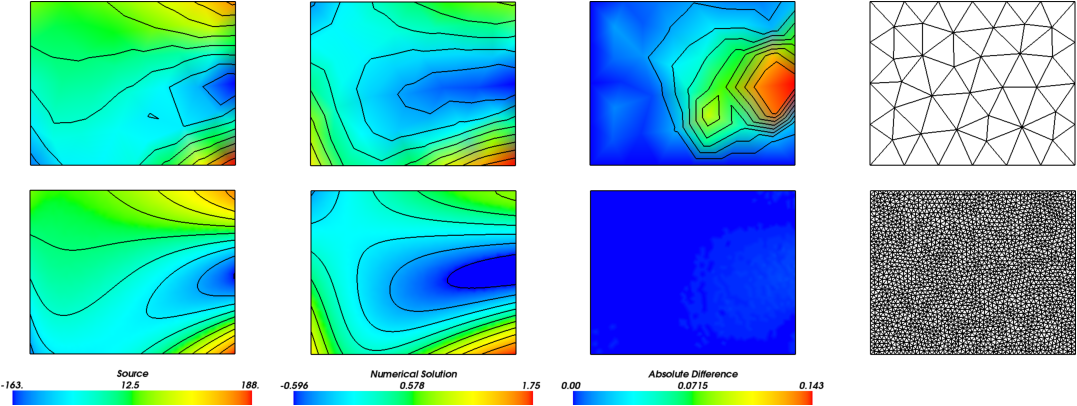
\includegraphics[width=\textwidth]{MMS}     
  \end{center}

{\tiny From left to right: source term for
the method of manufactured solutions advection-diffusion test case, the numerical solution calculated using a piecewise-linear
Galerkin discretisation, the absolute difference between the analytical and numerical solutions, the meshes used to compute the
previous images with average mesh spacings, $h$, of $0.08$ (top) and $0.01$ (bottom).}

\end{frame}

\begin{frame}{Method of manufactured solution: does our software work?}
  
  \begin{center}
    % \renewcommand{\tabcolsep}{1cm} \renewcommand{\arraystretch}{1.0}
    \begin{tabular}{@{\hspace{0.05cm}}c@{\hspace{0.05cm}} | @{\hspace{0.05cm}}c@{\hspace{0.05cm}} @{\hspace{0.05cm}}c@{\hspace{0.05cm}}
        @{\hspace{0.05cm}}c@{\hspace{0.05cm}} @{\hspace{0.05cm}}c@{\hspace{0.05cm}}
        @{\hspace{0.05cm}}c@{\hspace{0.05cm}}} 
      \hline
      $h_1\rightarrow h_2$ \ & $0.08 \rightarrow 0.04$ \ & $0.04\rightarrow
      0.02$ \ & $0.02\rightarrow 0.01$ \ & $0.01\rightarrow 0.005$\\ \hline 
      $n$ (CV)   \ &   2.42   \  &   2.00    \ &  1.43 \ & 0.97 \\ \hline 
      $n$ (P1) \ &    2.03    \  &   1.91    \ &  2.08 \ & 2.12 \\ \hline 
    \end{tabular} 
    \vspace{1ex}
  \end{center}
  
  {\small The difference between the analytical and numerical solutions
  using a first-order control volume (CV) discretisation and a second-order piecewise-linear Galerkin (P1) discretisation are
  calculated in the $L^2$ norm.  The ratio between these on two spatial mesh resolutions, $h_1$ and $h_2$, are used to estimate the
  order of spatial convergence of the model for this problem. The expected order of convergence, or better, is observed for both
  spatial discretisations.}


\end{frame}

\begin{frame}{Test driven development}
  
  Core commandments of the cult:
  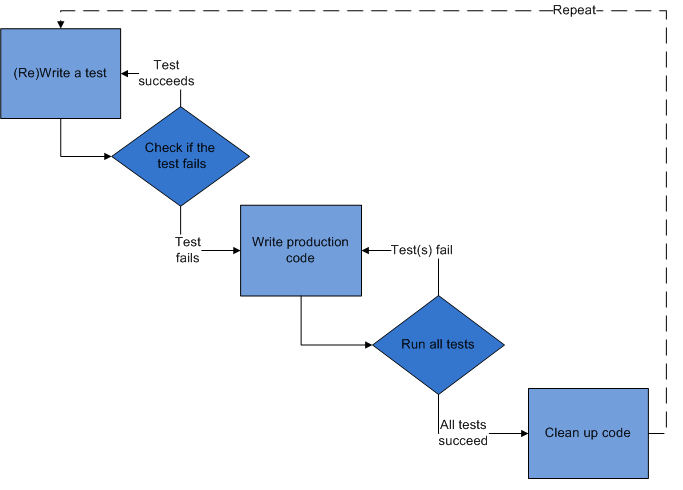
\includegraphics[height=.8\textheight]{Test-driven_development.PNG} 
  
  \tiny Image from \url{http://en.wikipedia.org/wiki/File:Test-driven_development.PNG}
\end{frame}

\begin{frame}{Reality check: a test heirarchy}

  Fluidity at Imperial uses this heirarchy:

  \begin{enumerate}
  \item Unit tests - very fast
  \item Short tests $<$ 20s each
  \item Medium tests up to several minutes.
  \item Long tests - usually parallel, may take hours.
  \end{enumerate}
  
  \begin{itemize}
  \item  Users are expected to run unit tests and short tests locally.
  \item  Everything up to medium is run on every trunk commit and can be requested
  for any branch commit.
  \item Long tests run on trunk on a rolling basis.
  \end{itemize}
  
\end{frame}

\begin{frame}{Even more real check: where to start}
  
  \begin{enumerate}
  \item create a test target in your build system (e.g. \texttt{make test})
  \item add unit tests using your favourite unit test framework.
  \item add verification tests using your favourite scripting language.
  \item \texttt{make test}\ 
  \end{enumerate}

\end{frame}

\begin{frame}{Buildbot: test automation}
  
  \begin{center}
    
    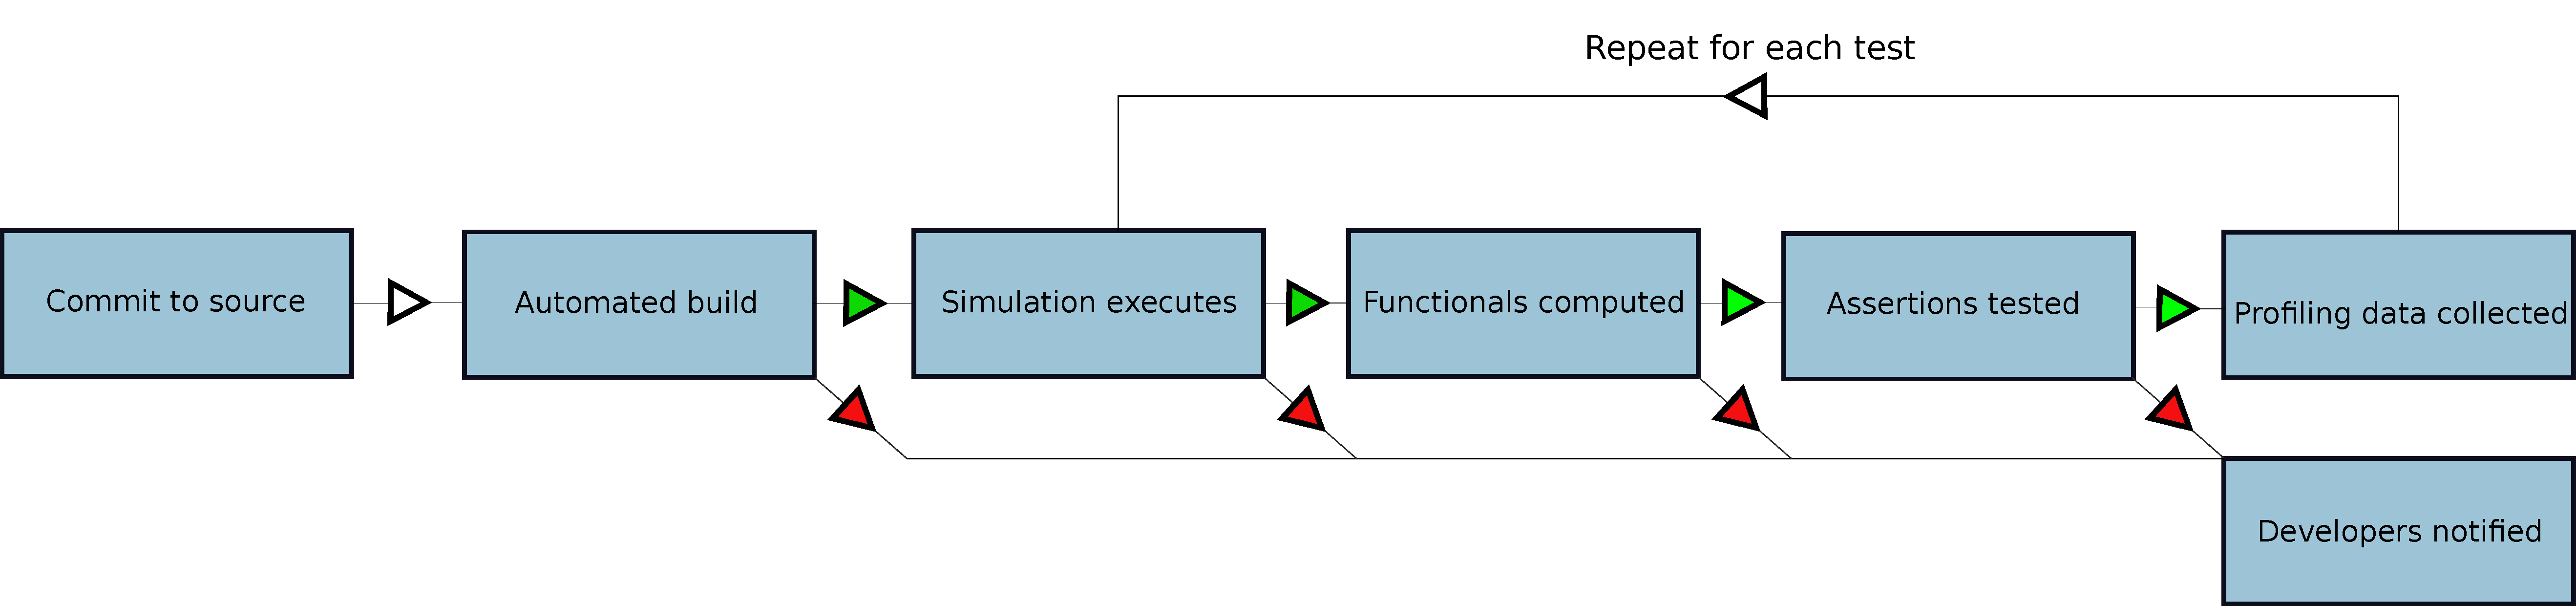
\includegraphics[width=\textwidth]{buildbot-simple.pdf}

  \end{center}

\end{frame}

\begin{frame}{Coverage tools: gcov}
  
  How do you know how good your tests are? If you're using gcc, then gcov can help!
  
  \begin{itemize}
  \item gcov (after using the right compiler options) provides information
    about how many times each file is called.
  \item lcov provides a graphical representation of this.
  \item However! Touching each line of code is necessary but not sufficient!
  \end{itemize}

\end{frame}

\end{document}
